%  30 Jan 2025 09:25:00
\documentclass{article}
\usepackage{geometry,booktabs,longtable,pdflscape,rotating,threeparttable,subcaption,graphicx,float,}
\usepackage{tabularx,colortbl,}
\usepackage[table]{xcolor}
\usepackage{hyperref}
\hypersetup{                           colorlinks=true,                   linkcolor={blue!50!black},                    filecolor={blue!50!black},                 urlcolor={blue!80!black},                     }                              \date{}
\geometry{verbose,letterpaper,lmargin=2.5cm,tmargin=2.5cm}

\begin{document}

\title{Illustrating the use of the latexlog package}
\maketitle
A descriptive analysis of the nlsw88.dta data
\section{Introduction}
This file provides examples of the use of the latexlog package.
The data used in this example is the nlsw88.dta data set, which is a sample data set provided with Stata.
\section{Summary Statistics}
\begin{figure}[H] 
\centering 
\caption{A scatterplot of wage vs. experience using the addfig subcommand} 
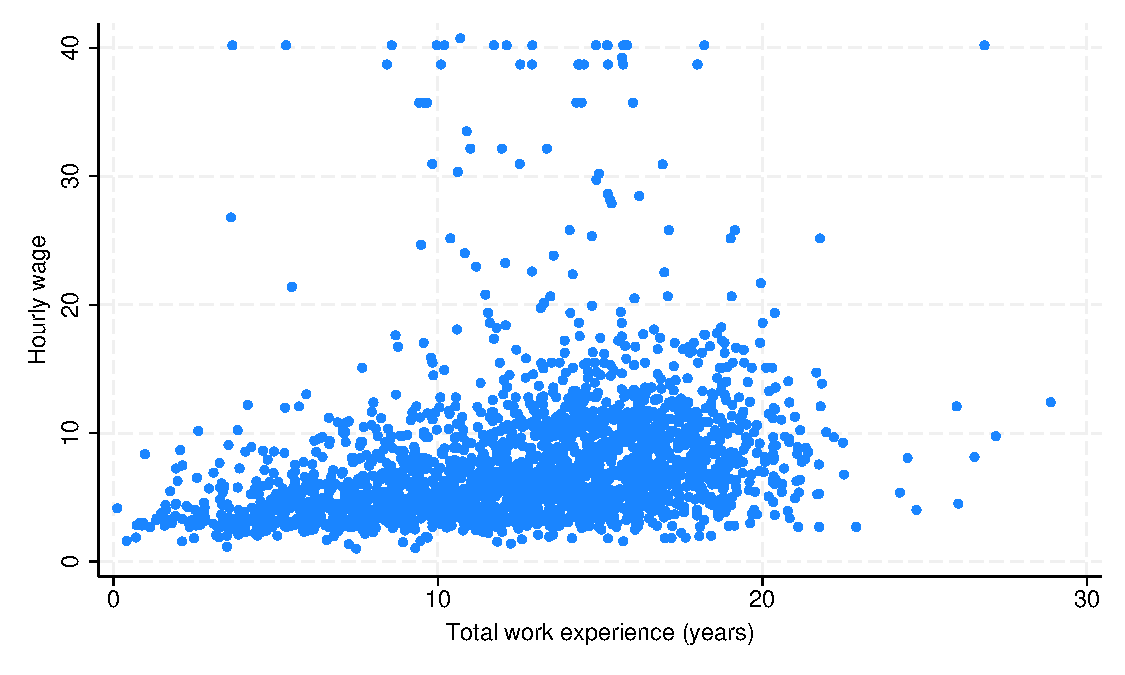
\includegraphics[width = .8\textwidth]{./figures/scatter_wage.pdf} \\ 
\begin{tabular}{p{6in}}  
\footnotesize \vspace{2pt} 
  \textbf{Notes:} Based on the nlsw88.dta data 
\end{tabular} 
\end{figure} 
\begin{figure}[H] 
\centering 
  \caption{Four Scatterplots of different variables vs. experience using the subfigure subcommand} 
\begin{subfigure}{.45\textwidth}
  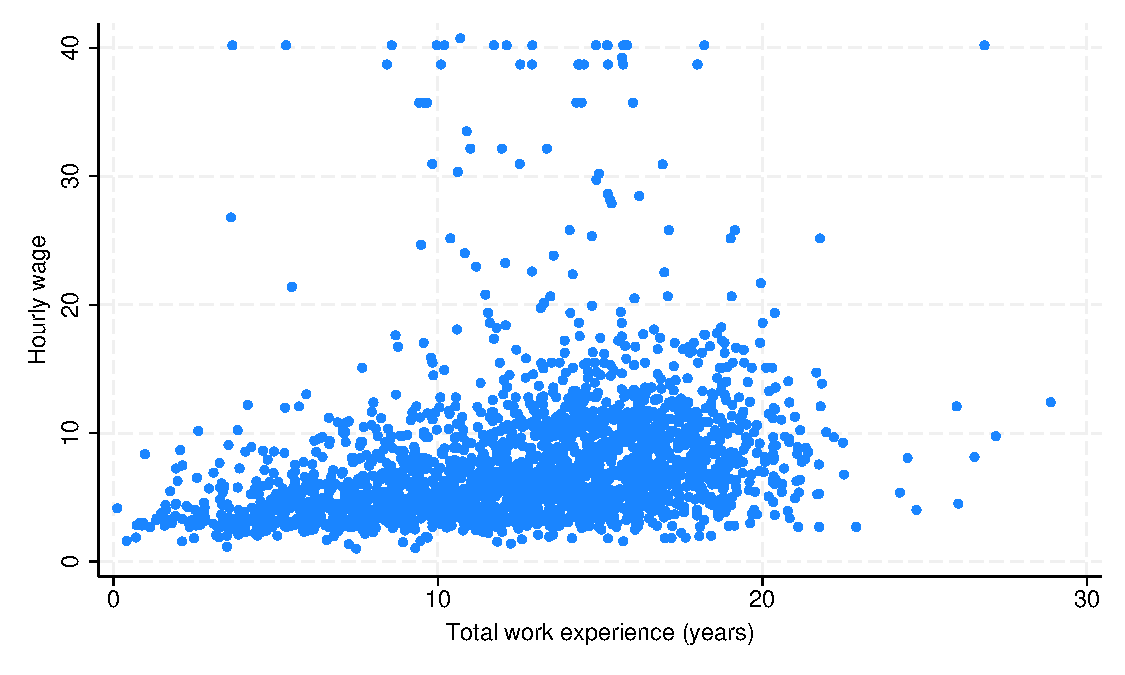
\includegraphics[width = 1.00\textwidth]{./figures/scatter_wage.pdf}  
  \caption{Hourly wage vs. experience}
\end{subfigure}
\begin{subfigure}{.45\textwidth}
  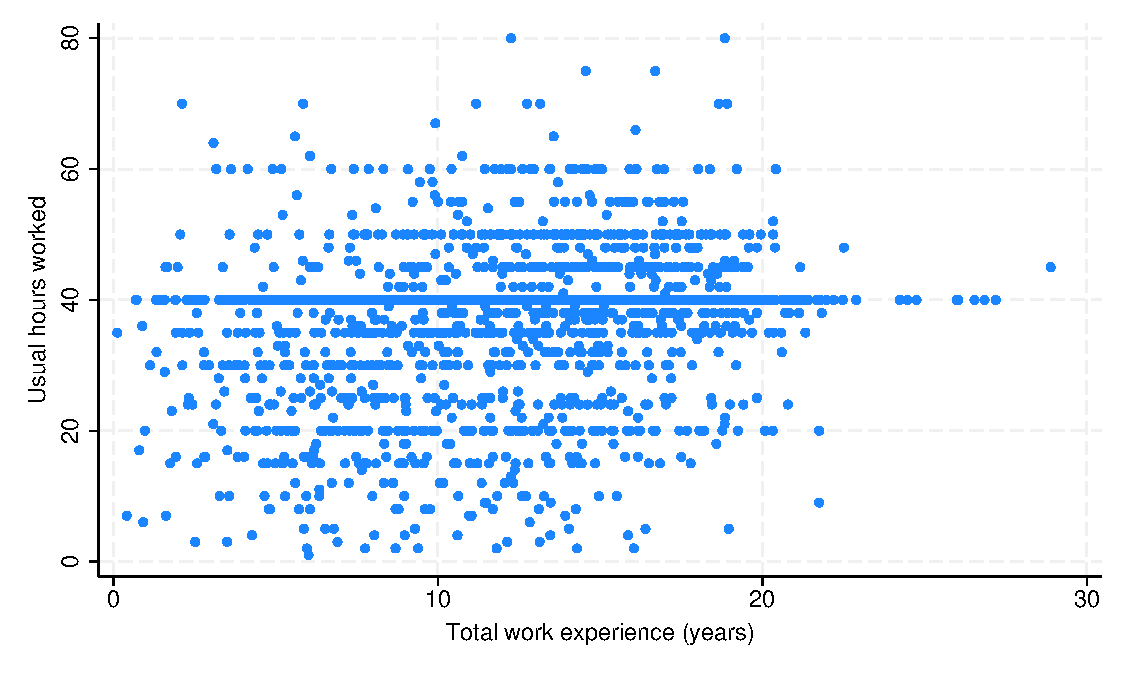
\includegraphics[width = 1.00\textwidth]{./figures/scatter_hours.pdf}  
  \caption{Usual hours worked vs. experience}
\end{subfigure}
\begin{subfigure}{.45\textwidth}
  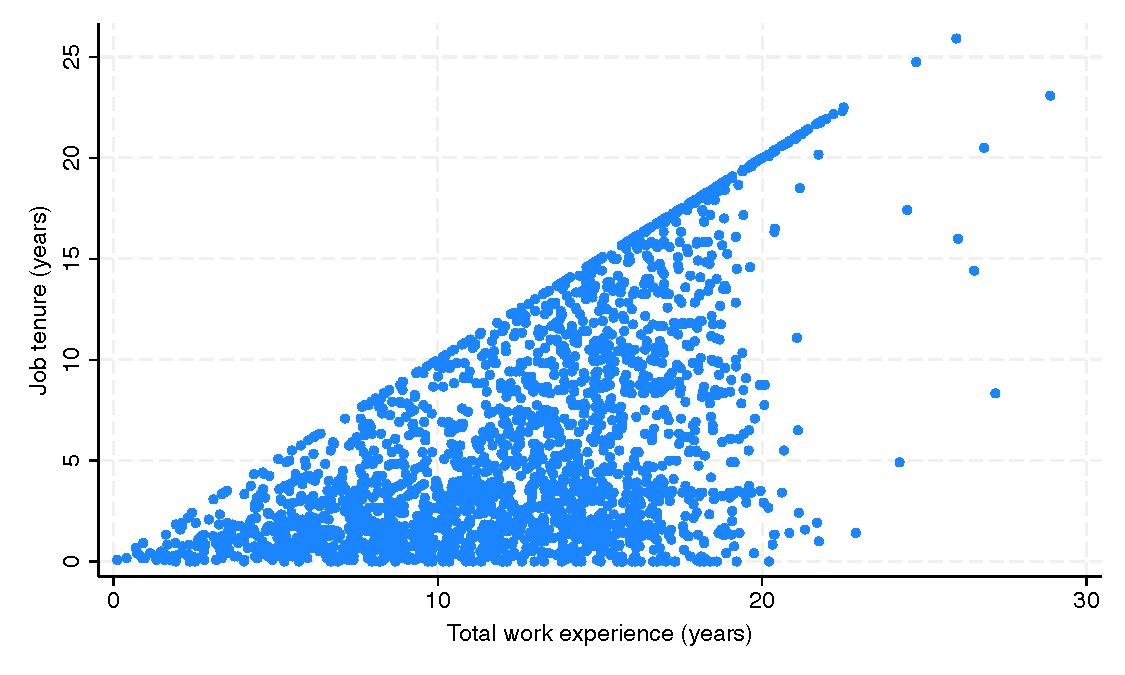
\includegraphics[width = 1.00\textwidth]{./figures/scatter_tenure.pdf}  
  \caption{Job tenure (years) vs. experience}
\end{subfigure}
\begin{subfigure}{.45\textwidth}
  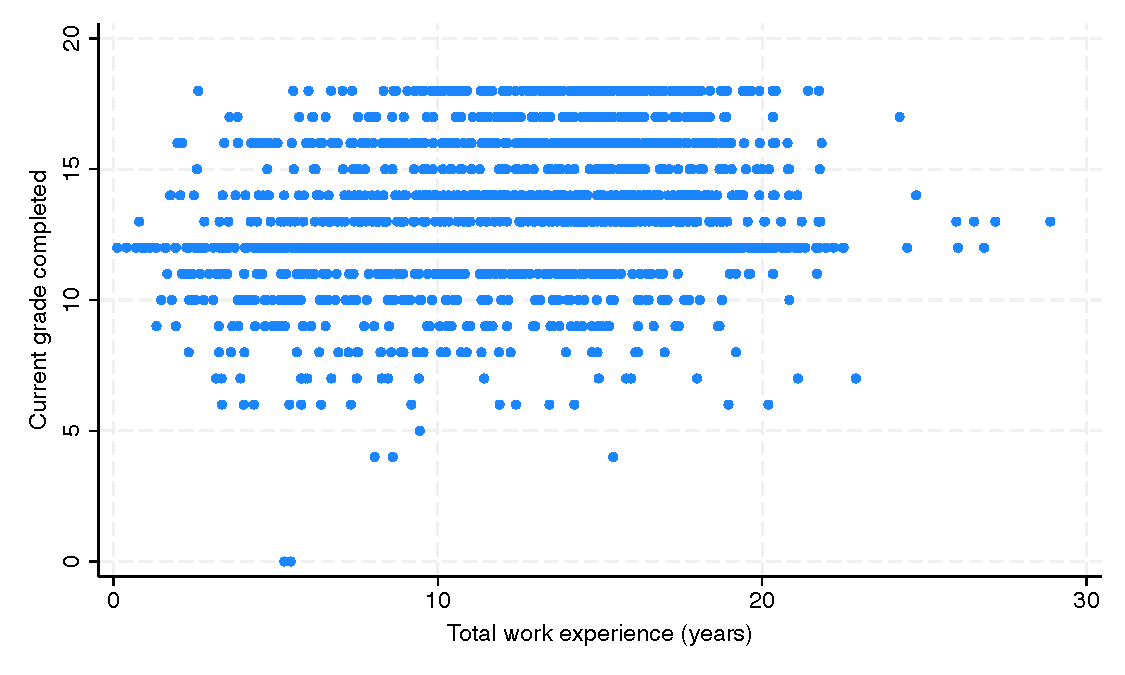
\includegraphics[width = 1.00\textwidth]{./figures/scatter_grade.pdf}  
  \caption{Current grade completed vs. experience}
\end{subfigure}
\begin{tabular}{p{6in}}  
 \footnotesize 
 \textbf{Notes:} Based on the nlsw88.dta data 
\end{tabular} 
\end{figure} 
\begin{figure}[H] 
\centering 
  \caption{Four Scatterplots of different variables vs. experience using the subfigure subcommand} 
\begin{subfigure}{.3\textwidth}
  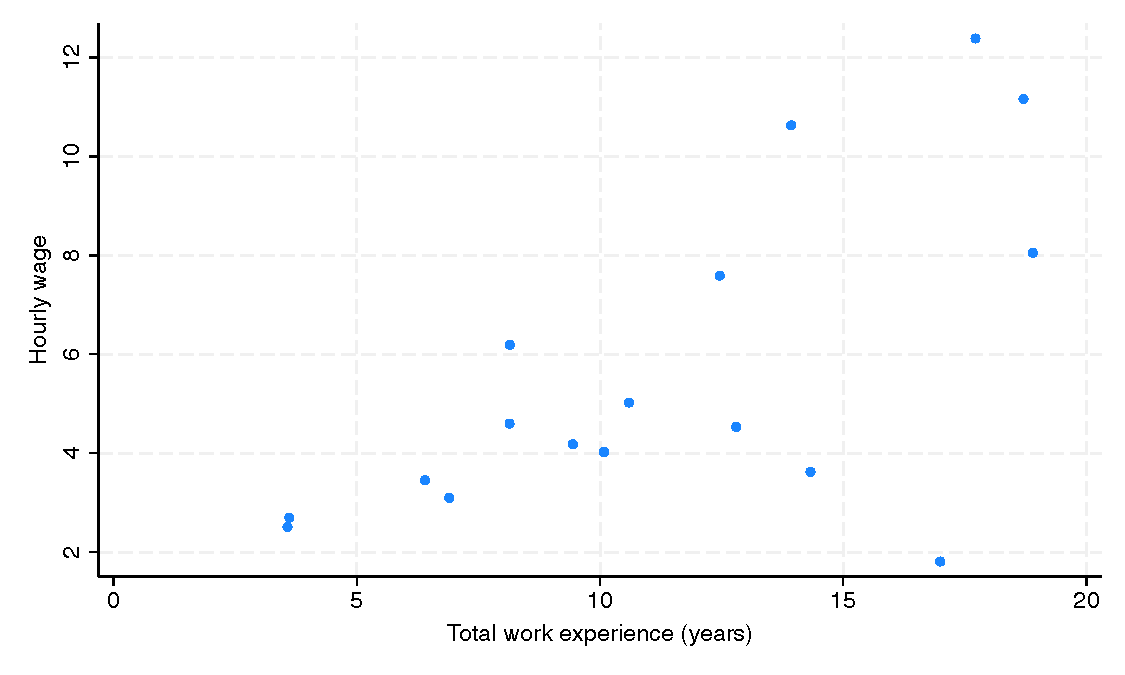
\includegraphics[width = 1.00\textwidth]{./figures/scatter_wage_ind1.pdf}  
  \caption{Wage vs. Total Experience for Ag/Forestry/Fisheries}
\end{subfigure}
\begin{subfigure}{.3\textwidth}
  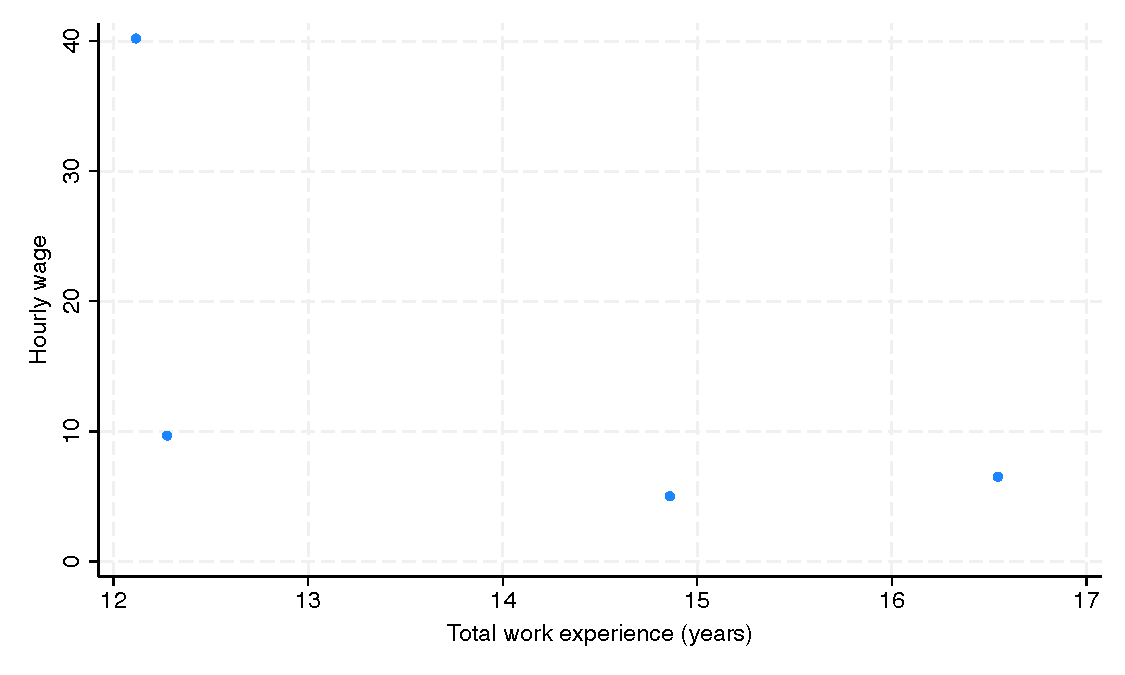
\includegraphics[width = 1.00\textwidth]{./figures/scatter_wage_ind2.pdf}  
  \caption{Wage vs. Total Experience for Mining}
\end{subfigure}
\begin{subfigure}{.3\textwidth}
  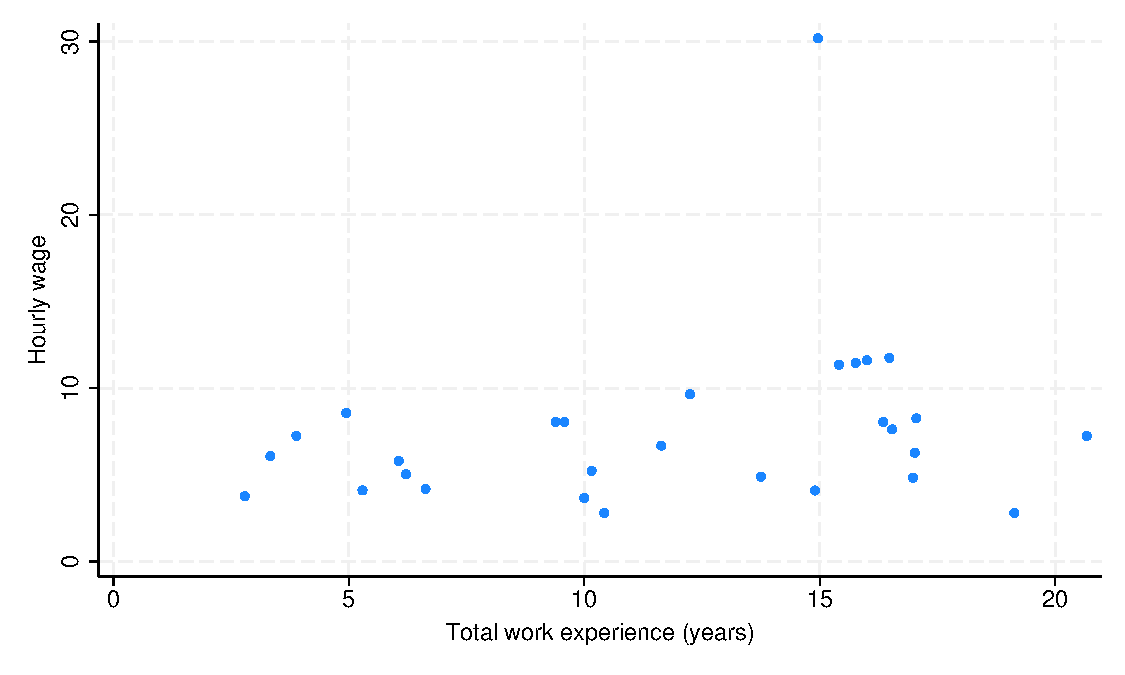
\includegraphics[width = 1.00\textwidth]{./figures/scatter_wage_ind3.pdf}  
  \caption{Wage vs. Total Experience for Construction}
\end{subfigure}
\begin{subfigure}{.3\textwidth}
  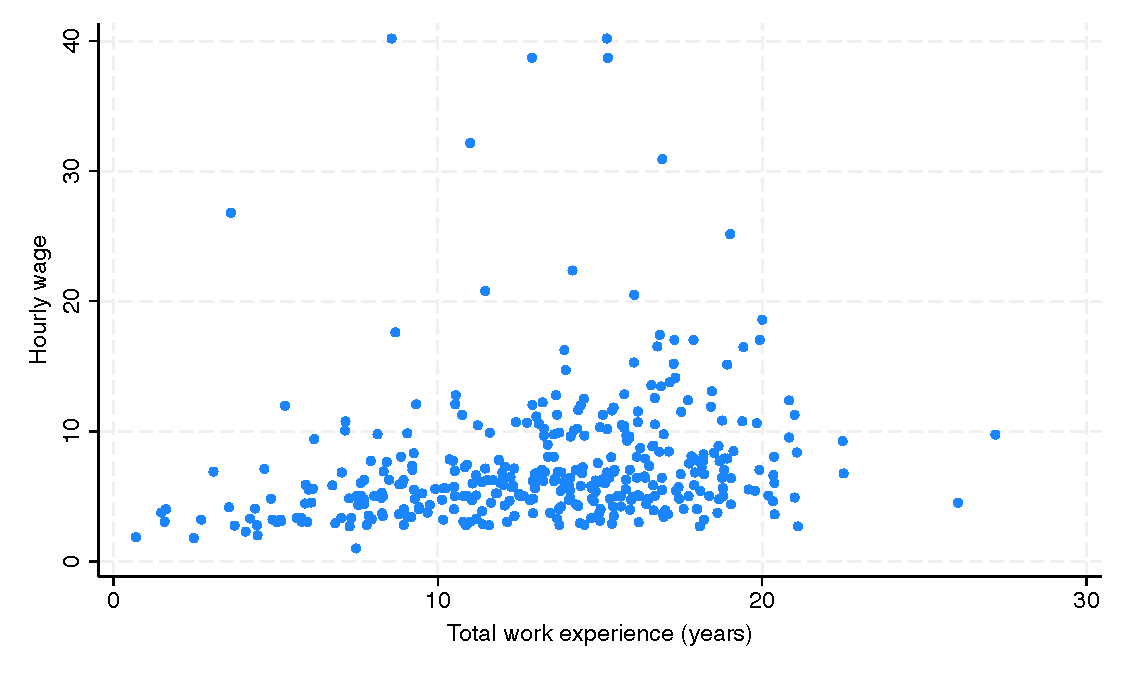
\includegraphics[width = 1.00\textwidth]{./figures/scatter_wage_ind4.pdf}  
  \caption{Wage vs. Total Experience for Manufacturing}
\end{subfigure}
\begin{subfigure}{.3\textwidth}
  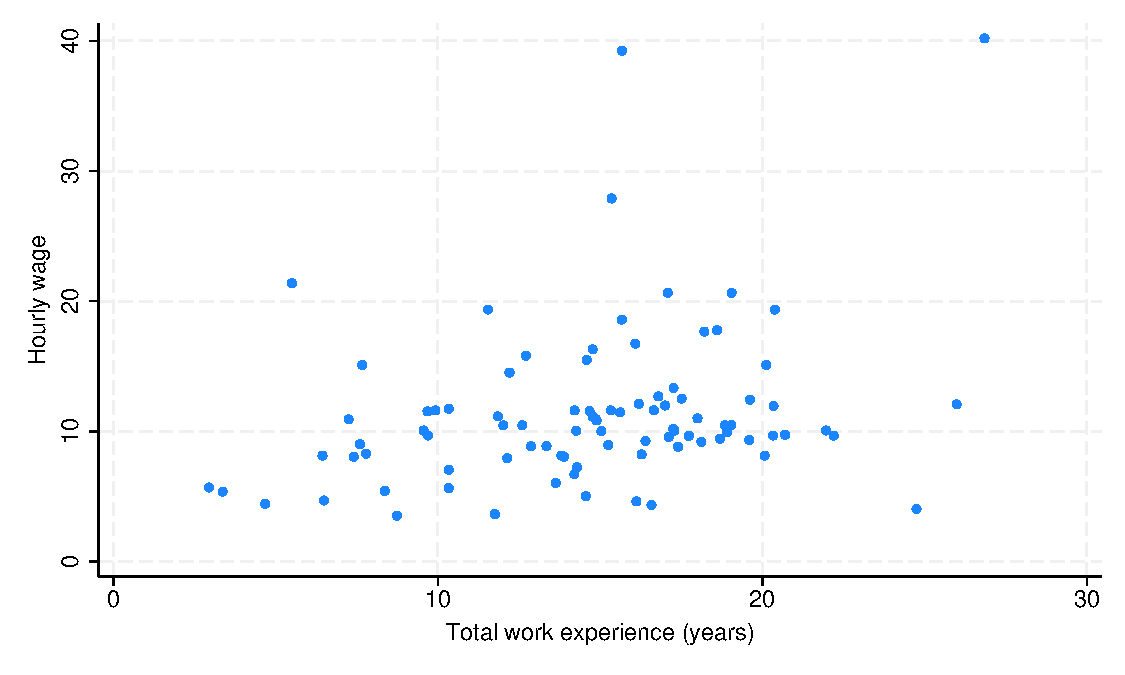
\includegraphics[width = 1.00\textwidth]{./figures/scatter_wage_ind5.pdf}  
  \caption{Wage vs. Total Experience for Transport/Comm/Utility}
\end{subfigure}
\begin{subfigure}{.3\textwidth}
  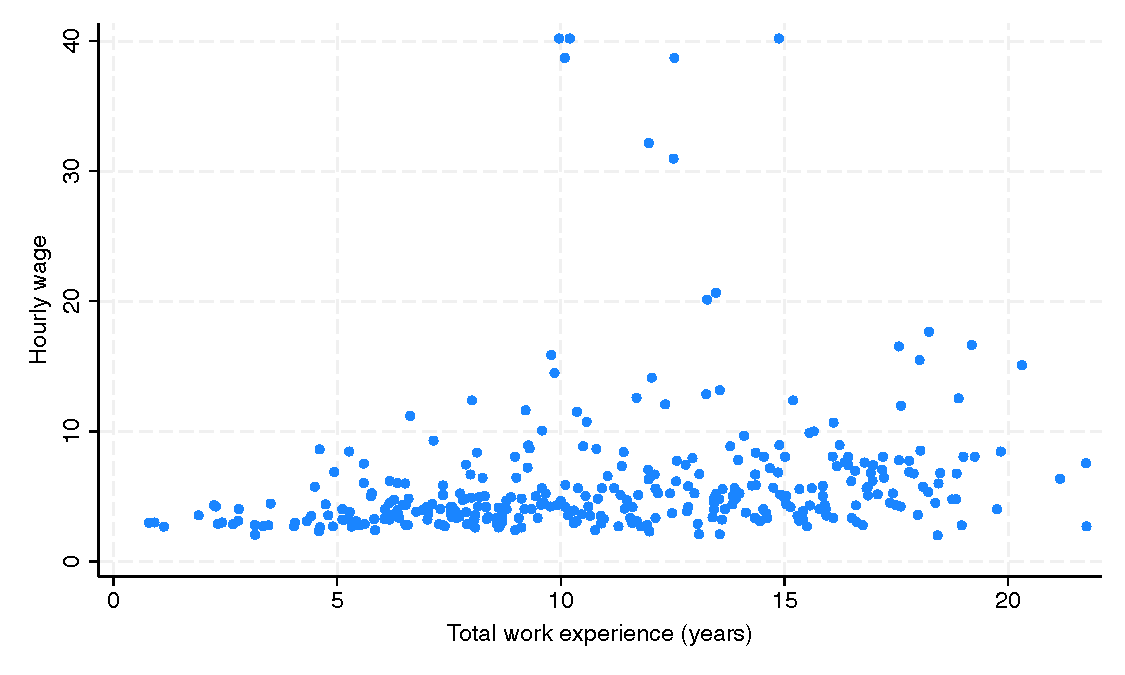
\includegraphics[width = 1.00\textwidth]{./figures/scatter_wage_ind6.pdf}  
  \caption{Wage vs. Total Experience for Wholesale/Retail trade}
\end{subfigure}
\begin{subfigure}{.3\textwidth}
  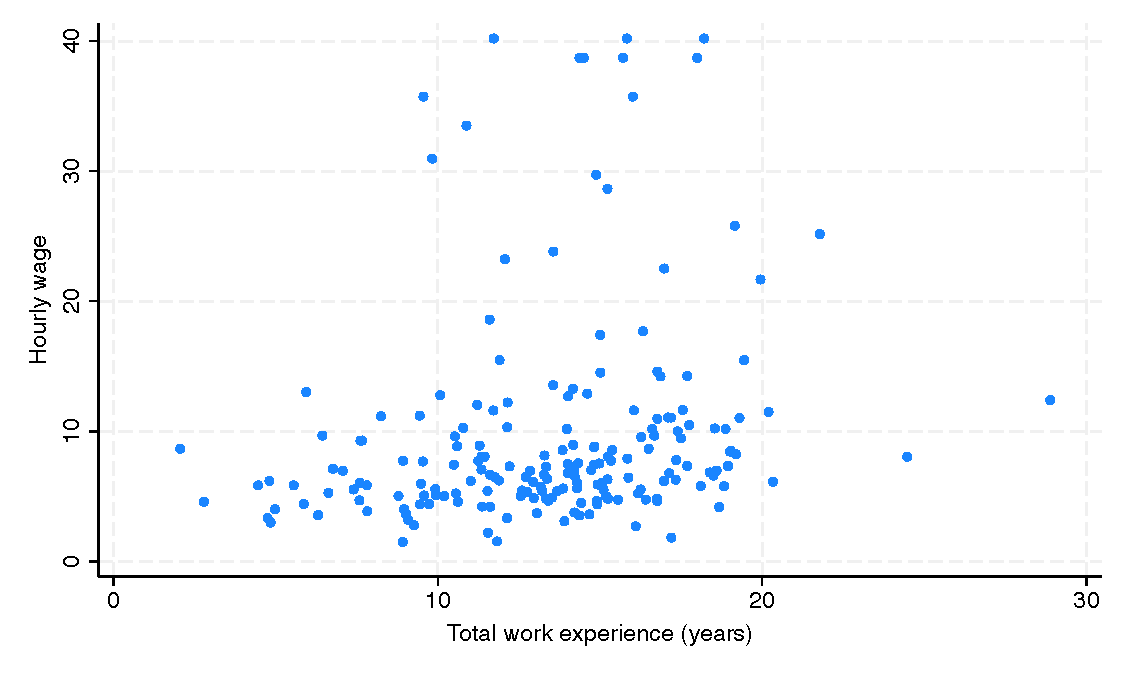
\includegraphics[width = 1.00\textwidth]{./figures/scatter_wage_ind7.pdf}  
  \caption{Wage vs. Total Experience for Finance/Ins/Real estate}
\end{subfigure}
\begin{subfigure}{.3\textwidth}
  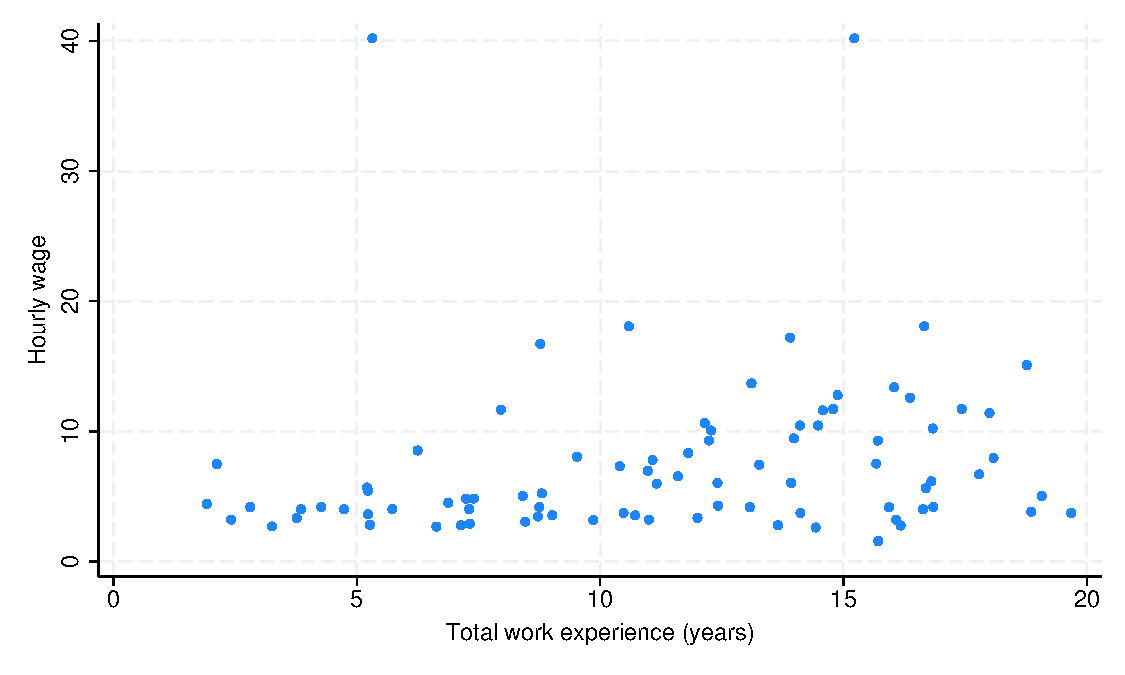
\includegraphics[width = 1.00\textwidth]{./figures/scatter_wage_ind8.pdf}  
  \caption{Wage vs. Total Experience for Business/Repair svc}
\end{subfigure}
\begin{subfigure}{.3\textwidth}
  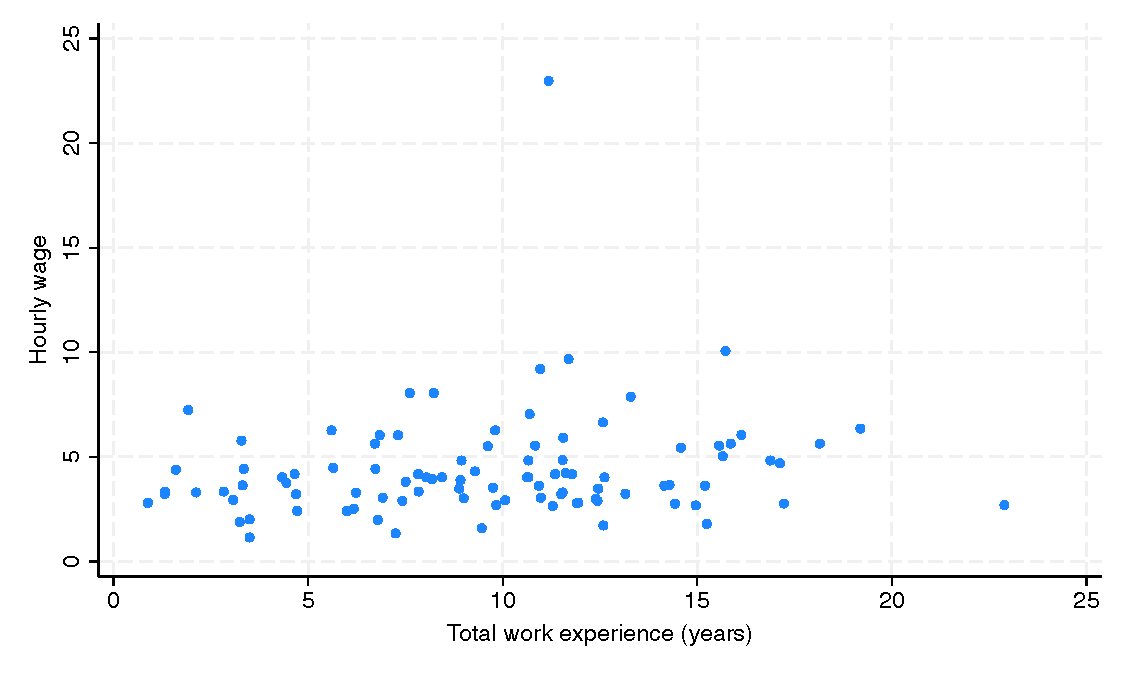
\includegraphics[width = 1.00\textwidth]{./figures/scatter_wage_ind9.pdf}  
  \caption{Wage vs. Total Experience for Personal services}
\end{subfigure}
\begin{subfigure}{.3\textwidth}
  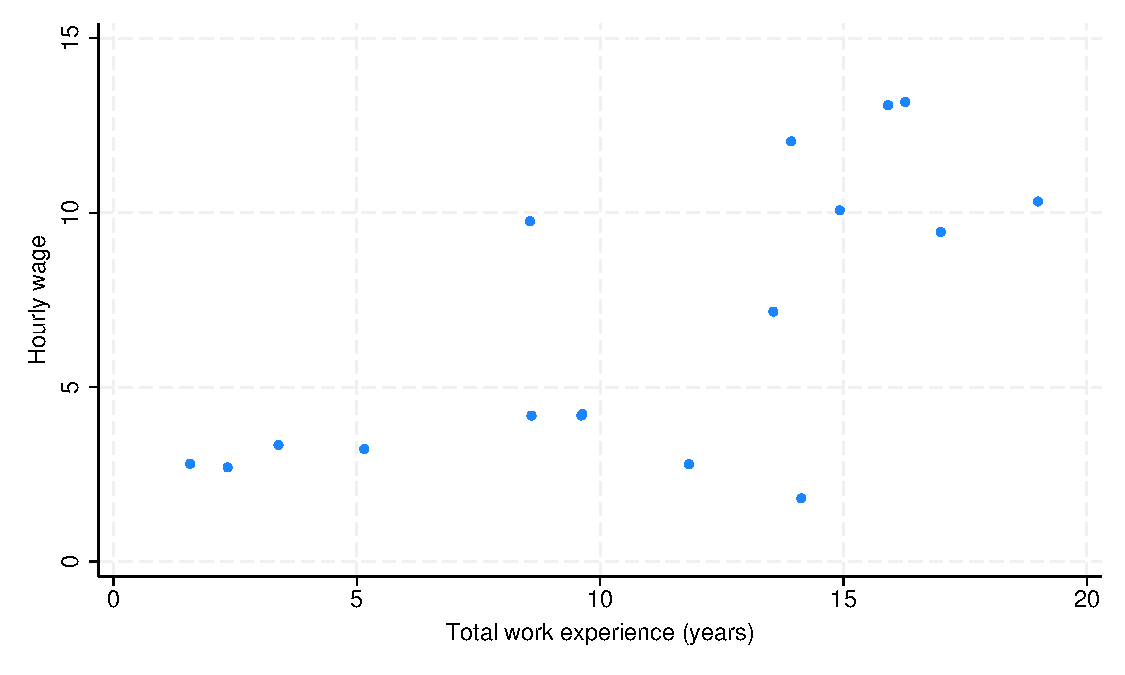
\includegraphics[width = 1.00\textwidth]{./figures/scatter_wage_ind10.pdf}  
  \caption{Wage vs. Total Experience for Entertainment/Rec svc}
\end{subfigure}
\begin{subfigure}{.3\textwidth}
  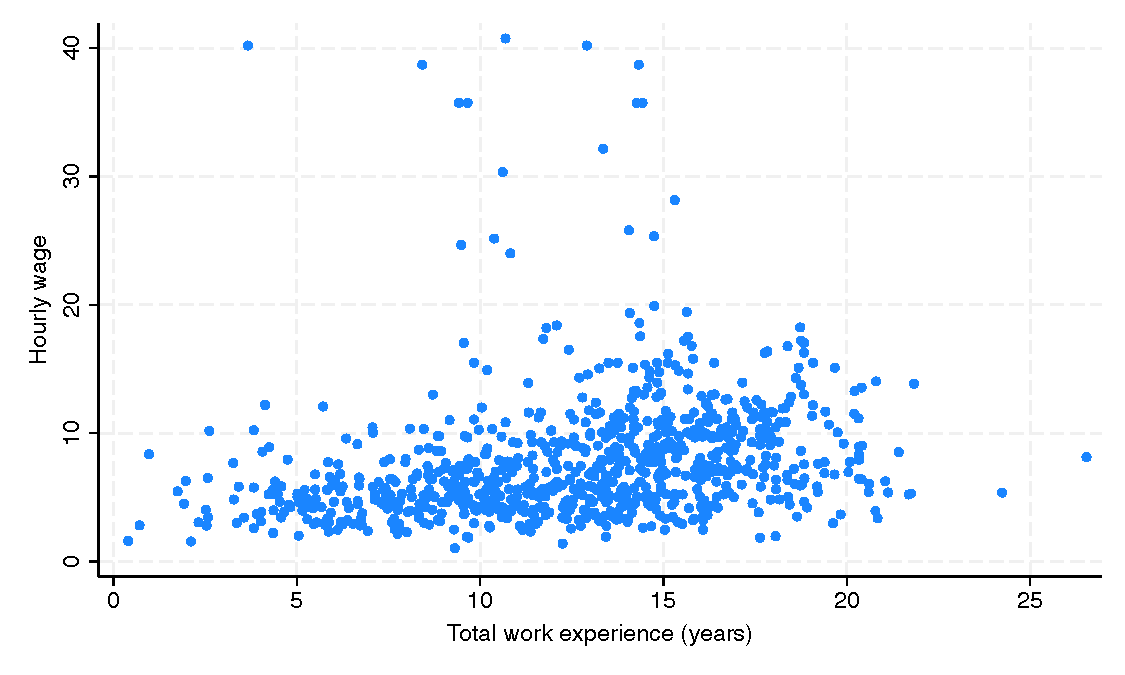
\includegraphics[width = 1.00\textwidth]{./figures/scatter_wage_ind11.pdf}  
  \caption{Wage vs. Total Experience for Professional services}
\end{subfigure}
\begin{subfigure}{.3\textwidth}
  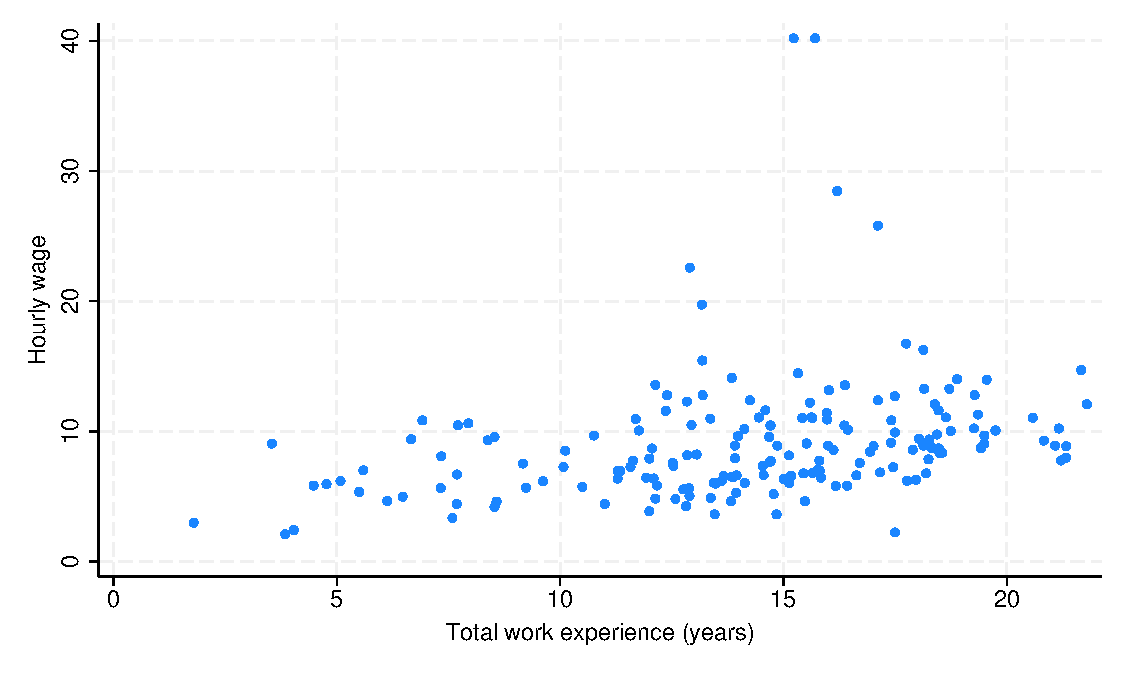
\includegraphics[width = 1.00\textwidth]{./figures/scatter_wage_ind12.pdf}  
  \caption{Wage vs. Total Experience for Public administration}
\end{subfigure}
\begin{tabular}{p{6in}}  
 \footnotesize 
 \textbf{Notes:} Based on the nlsw88.dta data 
\end{tabular} 
\end{figure} 
\clearpage\pagebreak
\section{Saving Tables with latexlog}
Since latexlog operates directly on a tex file, it is easy to save 
tables created with the \textbf{esttab} command or other commands that 
produce latex output that is appended to a file.
Here is an example of saving a table created with the esttab command:
 
\vspace{10pt}
\begin{table}[htbp]\centering
\def\sym#1{\ifmmode^{#1}\else\(^{#1}\)\fi}
\caption{Table using Stata "esttab" command to directly append to the log file}
\begin{tabular}{l*{1}{c}}
\toprule
            &\multicolumn{1}{c}{(1)}\\
            &\multicolumn{1}{c}{logwage}\\
\midrule
ttl\_exp     &      0.0480\sym{***}\\
            &     (19.76)         \\
\addlinespace
\_cons      &       1.267\sym{***}\\
            &     (39.07)         \\
\midrule
\(N\)       &        2246         \\
\bottomrule
\multicolumn{2}{l}{\footnotesize \textit{t} statistics in parentheses}\\
\multicolumn{2}{l}{\footnotesize \sym{*} \(p<0.05\), \sym{**} \(p<0.01\), \sym{***} \(p<0.001\)}\\
\end{tabular}
\end{table}

\vspace{10pt}
Stata's table command is very flexible and powerful. 
The following example creates a twoway table of the number workers in each occupation and union category 
using Stata's \textbf{table} command. 
This table is then saved to the log file using the \textbf{collect export} subcommand.
\begin{table}[htbp] 
\centering 
\begin{threeparttable} 
\caption{Table using Stata table command and latexlog collect export subcommand} 

\centering
\begin{tabular}{lll}
\toprule
\multicolumn{1}{c}{} &
  \multicolumn{2}{c}{Union worker} \\
\multicolumn{1}{c}{} &
  \multicolumn{1}{r}{Nonunion} &
  \multicolumn{1}{r}{Union} \\
\midrule
\multicolumn{1}{l}{Occupation} &
  \multicolumn{1}{r}{} &
  \multicolumn{1}{r}{} \\
\multicolumn{1}{l}{\hspace{1em}Professional/Technical} &
  \multicolumn{1}{r}{208} &
  \multicolumn{1}{r}{66} \\
\multicolumn{1}{l}{\hspace{1em}Managers/Admin} &
  \multicolumn{1}{r}{204} &
  \multicolumn{1}{r}{19} \\
\multicolumn{1}{l}{\hspace{1em}Sales} &
  \multicolumn{1}{r}{468} &
  \multicolumn{1}{r}{145} \\
\multicolumn{1}{l}{\hspace{1em}Clerical/Unskilled} &
  \multicolumn{1}{r}{70} &
  \multicolumn{1}{r}{5} \\
\multicolumn{1}{l}{\hspace{1em}Craftsmen} &
  \multicolumn{1}{r}{40} &
  \multicolumn{1}{r}{10} \\
\multicolumn{1}{l}{\hspace{1em}Operatives} &
  \multicolumn{1}{r}{128} &
  \multicolumn{1}{r}{83} \\
\multicolumn{1}{l}{\hspace{1em}Transport} &
  \multicolumn{1}{r}{19} &
  \multicolumn{1}{r}{1} \\
\multicolumn{1}{l}{\hspace{1em}Laborers} &
  \multicolumn{1}{r}{171} &
  \multicolumn{1}{r}{35} \\
\multicolumn{1}{l}{\hspace{1em}Farmers} &
  \multicolumn{1}{r}{1} &
  \multicolumn{1}{r}{} \\
\multicolumn{1}{l}{\hspace{1em}Farm laborers} &
  \multicolumn{1}{r}{6} &
  \multicolumn{1}{r}{1} \\
\multicolumn{1}{l}{\hspace{1em}Service} &
  \multicolumn{1}{r}{7} &
  \multicolumn{1}{r}{5} \\
\multicolumn{1}{l}{\hspace{1em}Household workers} &
  \multicolumn{1}{r}{} &
  \multicolumn{1}{r}{1} \\
\multicolumn{1}{l}{\hspace{1em}Other} &
  \multicolumn{1}{r}{87} &
  \multicolumn{1}{r}{89} \\
\bottomrule
\end{tabular}

 \footnotesize  
\textbf{Notes:} Command: table occupation union, nototals 
\end{threeparttable} 
\end{table}
\begin{table}[htbp] 
\centering 
\begin{threeparttable} 
\caption{Regression Table using Stata etable command and latexlog collect export subcommand} 

\centering
\begin{tabular}{lll}
\toprule
\multicolumn{1}{r}{} &
  \multicolumn{1}{c}{logwage} &
  \multicolumn{1}{c}{logwage} \\
\midrule
\multicolumn{1}{l}{Total work experience (years)} &
  \multicolumn{1}{r}{0.048} &
  \multicolumn{1}{r}{0.039} \\
\multicolumn{1}{l}{} &
  \multicolumn{1}{r}{(0.002)} &
  \multicolumn{1}{r}{(0.002)} \\
\multicolumn{1}{l}{Current grade completed} &
  \multicolumn{1}{r}{} &
  \multicolumn{1}{r}{0.081} \\
\multicolumn{1}{l}{} &
  \multicolumn{1}{r}{} &
  \multicolumn{1}{r}{(0.004)} \\
\multicolumn{1}{l}{Married} &
  \multicolumn{1}{r}{} &
  \multicolumn{1}{r}{-0.007} \\
\multicolumn{1}{l}{} &
  \multicolumn{1}{r}{} &
  \multicolumn{1}{r}{(0.022)} \\
\multicolumn{1}{l}{Intercept} &
  \multicolumn{1}{r}{1.267} &
  \multicolumn{1}{r}{0.325} \\
\multicolumn{1}{l}{} &
  \multicolumn{1}{r}{(0.032)} &
  \multicolumn{1}{r}{(0.060)} \\
\multicolumn{1}{l}{Number of observations} &
  \multicolumn{1}{r}{2246} &
  \multicolumn{1}{r}{2244} \\
\multicolumn{1}{l}{Adjusted R-squared} &
  \multicolumn{1}{r}{0.15} &
  \multicolumn{1}{r}{0.27} \\
\bottomrule
\end{tabular}

 \footnotesize  
\textbf{Notes:} Command: etable, estimates(model1 model2) mstat(N) mstat(r2\_a) 
\end{threeparttable} 
\end{table}

\end{document}
